\section{\method{}: Turning Hidden Knowledge into Better Decisions}
\label{sec:method}

In this section, we propose \method{}, a lightweight inference-time method that uses the probe's prediction to prefill the model's response with a short steering sentence, guiding the model to either solve directly or call a tool. This translates the internal signal identified in Section~\ref{sec:probing} into better tool-call decisions, requiring no model fine-tuning and no reasoning overhead.

\subsection{Method}

\method{} operates in three steps at inference time:

\paragraph{Step 1: Extract last hidden states.}
Given a task prompt, we run a single forward pass over the input tokens and extract the hidden states at the last token position. This is the standard prompt-encoding step that every LLM performs to get KV cache before autoregressive decoding begins, so hidden state extraction adds no additional forward passes.
\vspace{-5pt}
\paragraph{Step 2: Linear probe prediction.}
We apply the trained linear probe to all-layer hidden states, producing a probability $p$. A threshold $\tau$ converts this into a binary decision: if $p < \tau$, the task is predicted to be solvable without tools; otherwise, a tool call is predicted to be necessary. The threshold $\tau$ provides a single knob for controlling the accuracy--efficiency tradeoff: lower $\tau$ skips more tool calls (saves cost, risks missing necessary ones); higher $\tau$ preserves more tool calls (higher accuracy, fewer savings).
\vspace{-5pt}
\paragraph{Step 3: Prefill before generation.}
Based on the probe's prediction, we prepend a short steering sentence to the beginning of the model's response:
\begin{itemize}[leftmargin=*]
    \vspace{-3pt}
    \item If $p < \tau$ (tool unnecessary): ``\texttt{I can solve this directly without using a tool.}''
    \vspace{-3pt}
    \item If $p \geq \tau$ (tool necessary): ``\texttt{I need to use a tool for this question.}''
    \vspace{-3pt}
\end{itemize}
The model then continues generating from this prefill, producing either a direct answer or a tool call. This \emph{soft} prefill allows the model to override the suggestion if its own assessment disagrees. We also evaluate a \emph{hard} prefill mode that forces the output format (\texttt{\textbackslash boxed\{} for direct answers, tool-call JSON for tool use), leaving no room for the model to deviate (Table~\ref{tab:abl_prefill}, Appendix~\ref{app:ablation_prefill}).


\subsection{Main results}

Figures~\ref{fig:tradeoff} and~\ref{fig:tradeoff_llama} show the accuracy vs.\ tool-call tradeoff across six models.

\paragraph{\method{} outperforms the Prompt-only baseline.}
Compared to the Prompt-only baseline (gray), \method{} (green) is strictly better on Qwen models (Figure~\ref{fig:tradeoff}): it achieves higher accuracy at every tool-call budget, or equivalently, fewer tool calls at every accuracy level. Moreover, by sweeping the threshold $\tau$, \method{} traces a smooth tradeoff curve, providing fine-grained control over the operating point. In contrast, prompt engineering offers only a handful of discrete, fixed operating points with no way to interpolate between them. For Llama models (Figure~\ref{fig:tradeoff_llama}), soft prefill is partially ignored due to the bad instruction following; hard prefill restores full tradeoff control by forcing the output format.

\begin{figure*}[t]
\centering
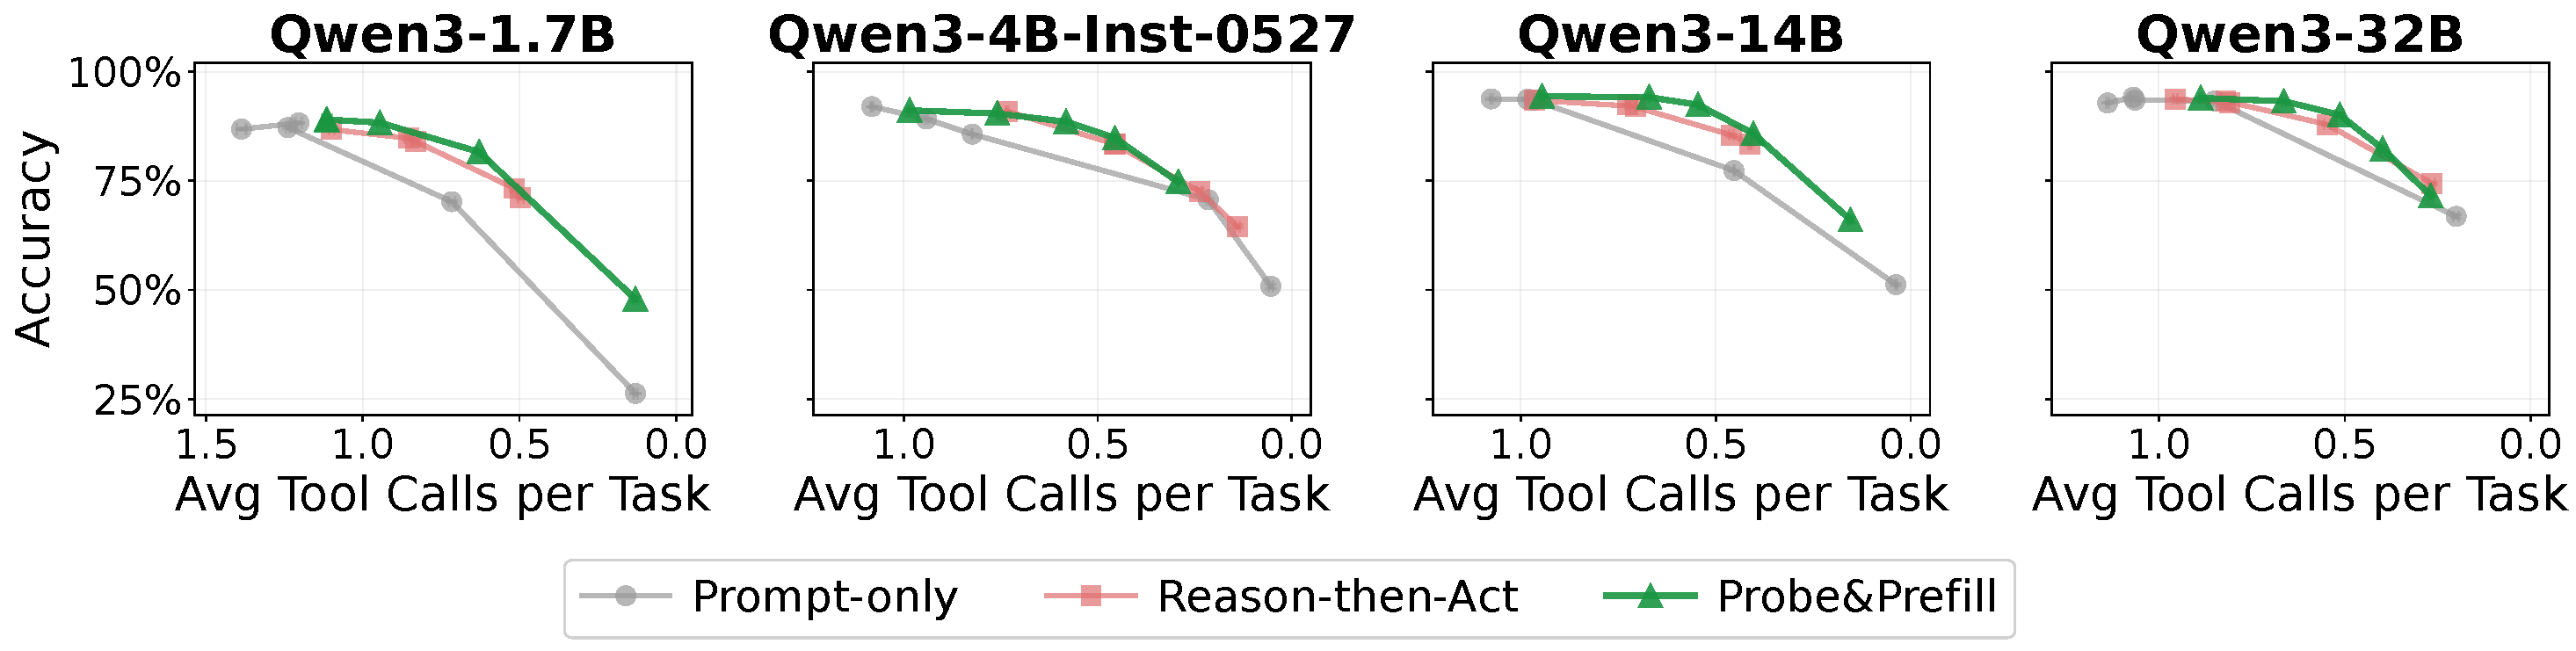
\includegraphics[width=\textwidth]{figures/fig2a_qwen.pdf}
\vspace{-15pt}
\caption{Accuracy vs.\ total tool calls for Qwen models. \method{} sweeps threshold $\tau$ from 0.1 to 0.9, achieving a strictly better tradeoff than both baselines.}
\vspace{-5pt}
\label{fig:tradeoff}
\end{figure*}

\begin{figure*}[t]
\centering
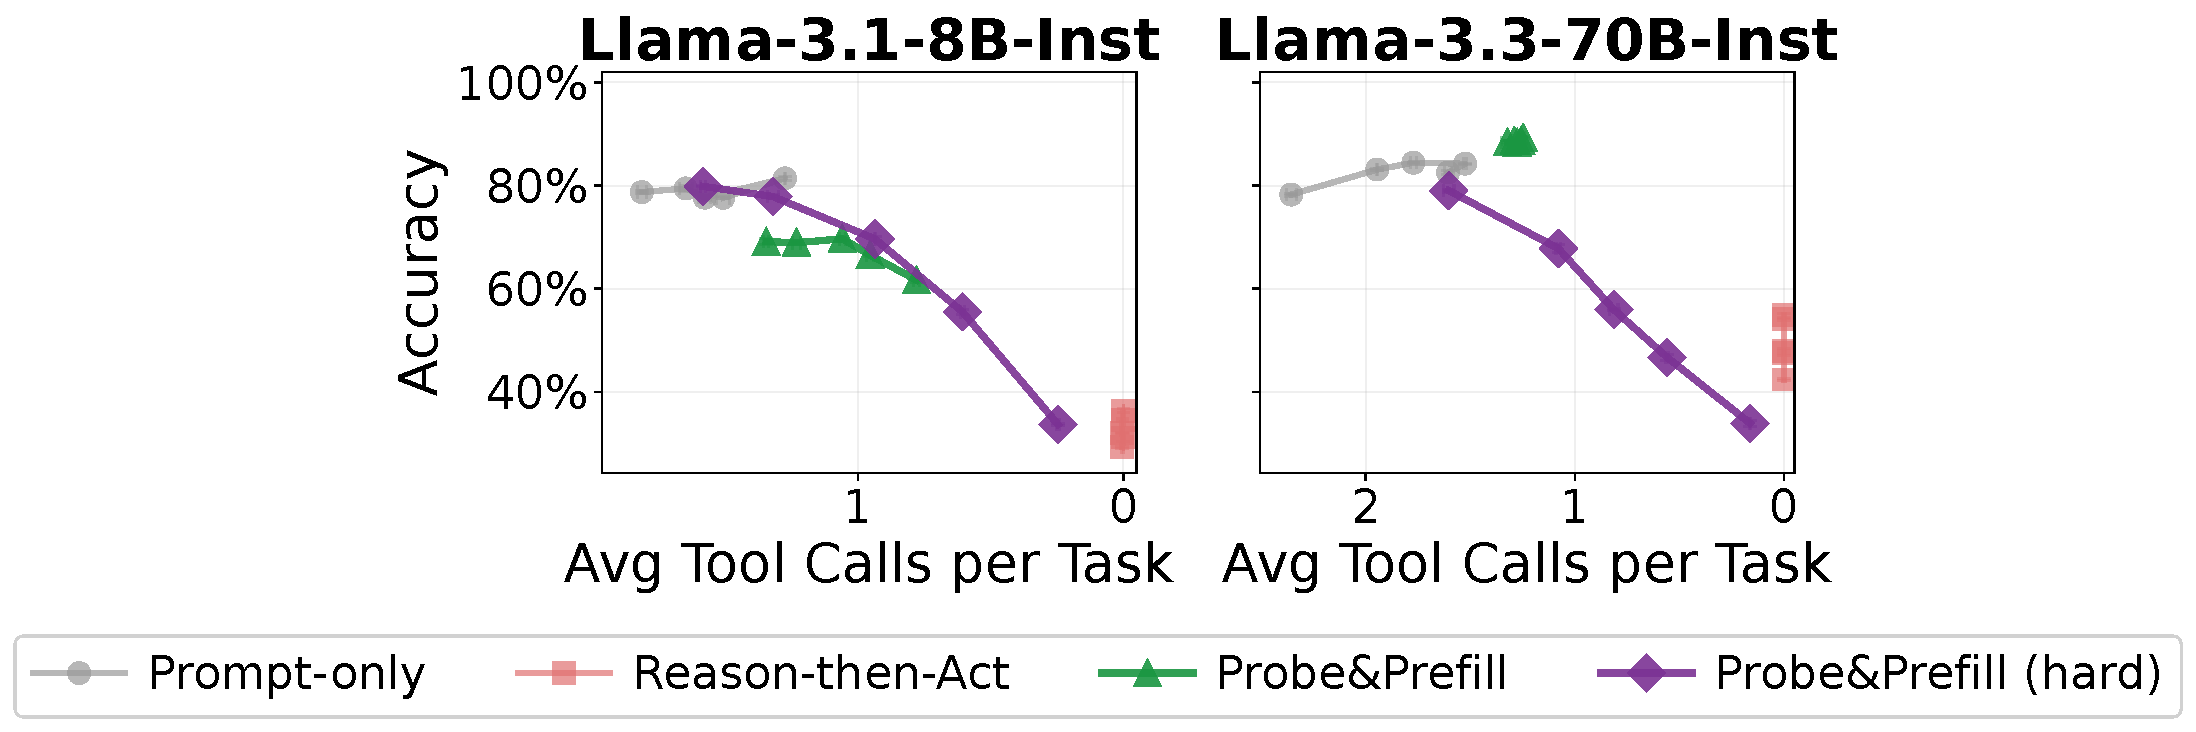
\includegraphics[width=0.8\textwidth]{figures/fig2b_llama.pdf}
\vspace{-5pt}
\caption{Accuracy vs.\ total tool calls for Llama models. Soft prefill (green) is partially ignored; hard prefill (purple) forces the output format and restores full tradeoff control.}
\vspace{-10pt}
\label{fig:tradeoff_llama}
\end{figure*}


\vspace{-5pt}
\paragraph{\method{} outperforms Reason-then-Act.}
\method{} also outperforms the Reason-then-Act baseline (red) in most cases, despite requiring no additional reasoning tokens. Reasoning asks the model to verbally assess tool necessity before acting, yet the probe's prediction from the pre-generation hidden state is more accurate than the model's own verbalized assessment. This suggests that reasoning about tool necessity is largely superficial: it does not improve the model's underlying decision beyond what is already encoded in its hidden states before any reasoning takes place. A striking example comes from the Llama models, where reasoning completely collapses tool calling (the red line in Figure~\ref{fig:tradeoff_llama} drops to near-zero tool calls with large accuracy loss), yet \method{} still achieves strong performance by reading the hidden state directly.
\vspace{-5pt}
\paragraph{Adaptive tool-call reduction.}
A key advantage of \method{} over the baselines is \emph{adaptive} reduction: the probe selectively skips easy calls while preserving hard ones. Table~\ref{tab:adaptive_reduction} compares the accuracy cost per saved call across all prompt strategies and \method{} ($\tau$=0.5), averaged over six models. Every baseline shows strongly negative costs, meaning each saved call comes at a significant accuracy penalty, especially on hard tasks. \method{} achieves the lowest cost across all difficulty levels ($-$1.6 easy, $-$3.4 hard), reducing tool calls with minimal accuracy loss. 

\begin{table*}[h]
\caption{Accuracy cost per saved call ($\frac{\Delta\text{Acc}}{-\Delta\text{TC}}$), averaged across six models (threshold $\tau$ is set to 0.5 for \method{}). All changes are relative to Default~($\star$, Prompt-only). More negative $\frac{\Delta\text{Acc}}{-\Delta\text{TC}}$ means each saved call costs more accuracy. \method{} achieves lowest cost per saved call.}
\vspace{-5pt}
\label{tab:adaptive_reduction}
\centering
\footnotesize
\setlength{\tabcolsep}{1.8pt}
\begin{tabular}{l rrr rrr rrr rrr}
\toprule
& \multicolumn{3}{c}{Easy} & \multicolumn{3}{c}{Medium} & \multicolumn{3}{c}{Hard} & \multicolumn{3}{c}{Overall} \\
\cmidrule(lr){2-4} \cmidrule(lr){5-7} \cmidrule(lr){8-10} \cmidrule(lr){11-13}
Method & $\Delta$Acc & $\Delta$TC & $\frac{\Delta\text{Acc}}{-\Delta\text{TC}}$ & $\Delta$Acc & $\Delta$TC & $\frac{\Delta\text{Acc}}{-\Delta\text{TC}}$ & $\Delta$Acc & $\Delta$TC & $\frac{\Delta\text{Acc}}{-\Delta\text{TC}}$ & $\Delta$Acc & $\Delta$TC & $\frac{\Delta\text{Acc}}{-\Delta\text{TC}}$ \\
\midrule
Necessary (N)     & $-$0.3  & $-$0.09 & $-$3.5  & $-$0.7  & $-$0.04 & $-$17.9 & $-$1.9  & $-$0.04 & $-$44.4 & $-$1.0  & $-$0.06 & $-$16.8 \\
Necessary + Reason-then-Act & $-$8.1  & $-$0.95 & $-$8.5  & $-$16.3 & $-$0.82 & $-$19.7 & $-$23.2 & $-$0.70 & $-$32.9 & $-$15.8 & $-$0.82 & $-$19.2 \\
Sparse (S)        & $-$6.3  & $-$0.55 & $-$11.3 & $-$7.9  & $-$0.47 & $-$16.9 & $-$11.1 & $-$0.35 & $-$31.5 & $-$8.4  & $-$0.46 & $-$18.4 \\
Sparse + Reason-then-Act    & $-$9.9  & $-$1.13 & $-$8.8  & $-$19.9 & $-$1.04 & $-$19.1 & $-$29.3 & $-$0.84 & $-$34.7 & $-$19.7 & $-$1.00 & $-$19.6 \\
No Tool (X)       & $-$18.1 & $-$0.72 & $-$25.2 & $-$26.7 & $-$0.72 & $-$36.9 & $-$41.4 & $-$0.69 & $-$60.4 & $-$28.7 & $-$0.71 & $-$40.5 \\
No Tool + Reason-then-Act   & $-$12.4 & $-$1.18 & $-$10.5 & $-$23.5 & $-$1.12 & $-$20.9 & $-$36.6 & $-$0.94 & $-$39.1 & $-$24.2 & $-$1.08 & $-$22.4 \\
\midrule
\method{}  (Ours)        & $-$1.1  & $-$0.66 & \textbf{$-$1.6}  & $-$3.4  & $-$0.54 & \textbf{$-$6.2}  & $-$0.8  & $-$0.24 & \textbf{$-$3.4}  & $-$1.7  & $-$0.48 & \textbf{$-$3.6} \\
\bottomrule
\end{tabular}
\end{table*}

\subsection{Additional experiments}

Since \method{} introduces a learned probe, it is important to verify that results are not artifacts of overfitting to the training environments or sensitive to hyperparameter choices. We conduct the following additional experiments (full details in the Appendix):
\begin{itemize}[leftmargin=*]
    \item \textbf{Complete per-model results} (Appendix~\ref{app:full_reduction}): Full numerical tables for all models, prompt modes, reasoning settings, and probe thresholds on single-hop tasks.
    \item \textbf{Multi-hop tasks} (Appendix~\ref{app:multihop}): On the 3 multi-hop environments, \method{} reduces tool calls by up to 75\% on Qwen models while maintaining or improving accuracy.
    \item \textbf{Out-of-distribution transfer} (Appendix~\ref{app:ood}): The probe trained on a subset of environments generalizes to held-out environments within the same category.
    \item \textbf{Ablation studies} (Appendix~\ref{app:ablations}): Soft vs.\ hard prefill, temperature scaling, layer selection, data efficiency, and regularization strength.
    \item \textbf{Inference overhead} (Appendix~\ref{app:overhead}): The probe adds $<$1ms per task on top of the standard prefill forward pass, with no additional model calls.
    \item \textbf{Real-world agentic search} (Appendix~\ref{app:search_o1}): On Search-o1 agentic benchmark, \method{} reduces search API calls by 20--56\% while matching or exceeding baseline accuracy.
    \item \textbf{SFT baseline comparison} (Appendix~\ref{app:sft}): Full fine-tuning improves accuracy but does not reliably reduce tool calls, and is orders of magnitude more expensive than \method{}.
\end{itemize}